\begin{sidewaysfigure}
	%	\centering
	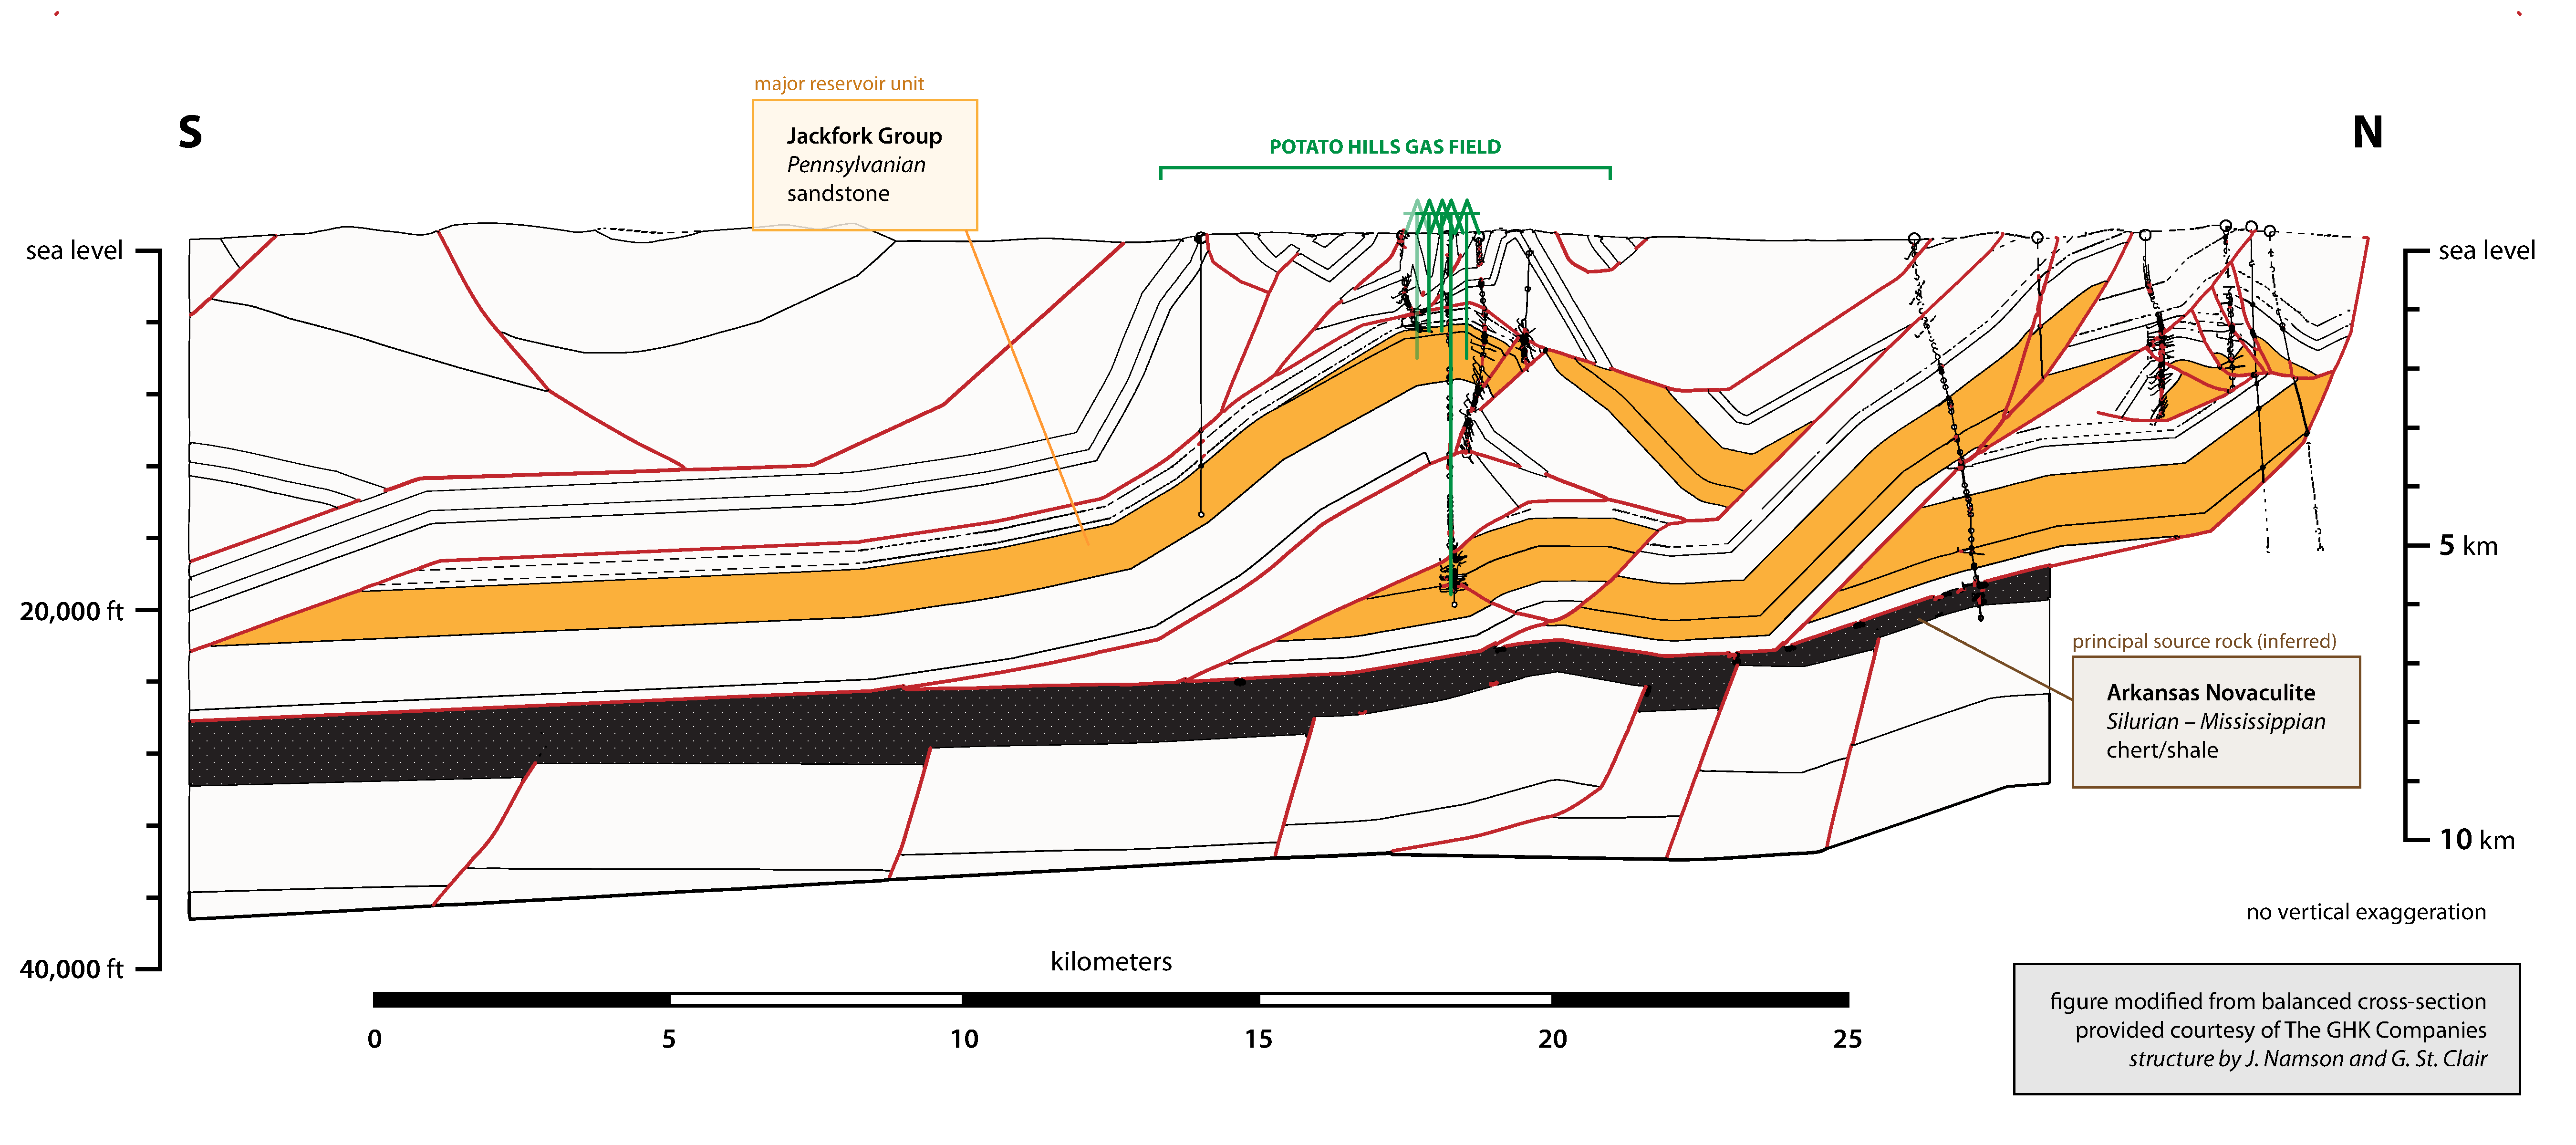
\includegraphics[width=\textwidth]{figures/FigA.2.pdf}
	\caption[Structural cross-section through the Potato Hills]{Balanced geologic cross-section through the Potato
		Hills for A--A$'$ (\autoref{fig:A:1}). The original cross-section on which this figure
		is based was provided courtesy of The GHK Companies. Structural
		interpretation was by J. Namson and G. St.\ Clair. Reservoir sands and
		presumed source are highlighted in orange and black, respectively.
		Faults are highlighted in red. Projections of studied wells onto the
		cross-section are shown in green.}
	\label{fig:A:2}
\end{sidewaysfigure}